% !TEX encoding = UTF-8 Unicode
\documentclass[
11pt,
master, % тип документа
subf, % подключить и настроить пакет subfig для вложенной нумерации рисунков
href, % подключить и настроить пакет hyperref
colorlinks=true, % цветные гиперссылки
%fixint=false % отключить прямые знаки интегралов
]{disser}
\usepackage[left=25mm, top=20mm, right=10mm, bottom=20mm]{geometry}
\usepackage[T2A]{fontenc}
\usepackage[utf8]{inputenc}
\usepackage[english,russian]{babel}
\usepackage{amsmath,amssymb,cmap} % cmap для кодировки шрифтов в pdf
\usepackage{pdfpages} % вставляем pdf файлы
\usepackage{indentfirst} % отделять первую строку раздела абзацным отступом
\usepackage{titletoc} % убираем отступ перед "Оглавление"
\usepackage{graphicx}
\usepackage{setspace}
\usepackage{verbatim} % для оформления кода
\usepackage{pdfsync} % установка соответствия документ - код
\graphicspath{{./Img/}}

\setlength\parindent{5ex} % абзацный отступ равный пяти строчным буквам основного шрифта
\setcounter{tocdepth}{2} % включать подсекции в оглавление
\linespread{1.3} % полуторный интервал

\pagestyle{footcenter}
\chapterpagestyle{footcenter}

\newcommand*{\PartDif}[2]{\frac{\partial #1}{\partial #2}}
\newcommand*{\PartDiff}[2]{\frac{\partial^2 #1}{\partial #2^2}}
\newcommand*{\PartD}[1]{\frac{\partial}{\partial #1}}
\newcommand*{\SR}[1]{\left[ #1 \right]}
\newcommand*{\Ap}[2]{\hat{#1}_{#2}}
\newcommand*{\Apr}[2]{#1_{#2}}

\begin{document}
	\pagestyle{empty}
	\begin{center}
		
		\noindent  Федеральное государственное бюджетное образовательное учреждение\\
		высшего профессионального образования\\
		
		Московский государственный технический университет им. Н.Э. Баумана \\
		Факультет <<Фундаментальные науки>>\bigskip\\
		
		\vfill
		
		Лабораторная работа №2\\
		по курсу «Вычислительная физика»\\
		
		
		\vfill
		\vfill
		\begin{flushright}
			\begin{tabular}{ll}
				Выполнил: & студент группы ФН4-82Б     \\
				& Хижик А.И. \\
				Проверил:  & доцент, к.физ.-мат.н.       \\
				& Хасаншин Р.Х.
			\end{tabular}
		\end{flushright}
		\vfill
		\begin{center}
			Москва, $2020$
		\end{center}
		
	\end{center}
	\pagebreak
	
	
	\pagestyle{plain}
	\tableofcontents

\section{Теоретическая часть}
\subsection*{Численное решение ДУ}
\begin{align}
        &\PartDif{u(x,t)}{t} = \PartD{x}\SR{D(x)\PartDif{u(x,t)}{x}} + f(x,t), \;\; 0 < x  < l, \;\; 0 < t < T, \label{eq:5}\\
        &u(x,t)\bigg|_{t = 0} = u_0(x), \label{eq:6}\\
        &u(0,t) = 0, \label{eq:7}\\
        &\PartDif{u}{x}(l,t) = 0. \label{eq:8}
\end{align}

\begin{figure}[h]
  \centering
  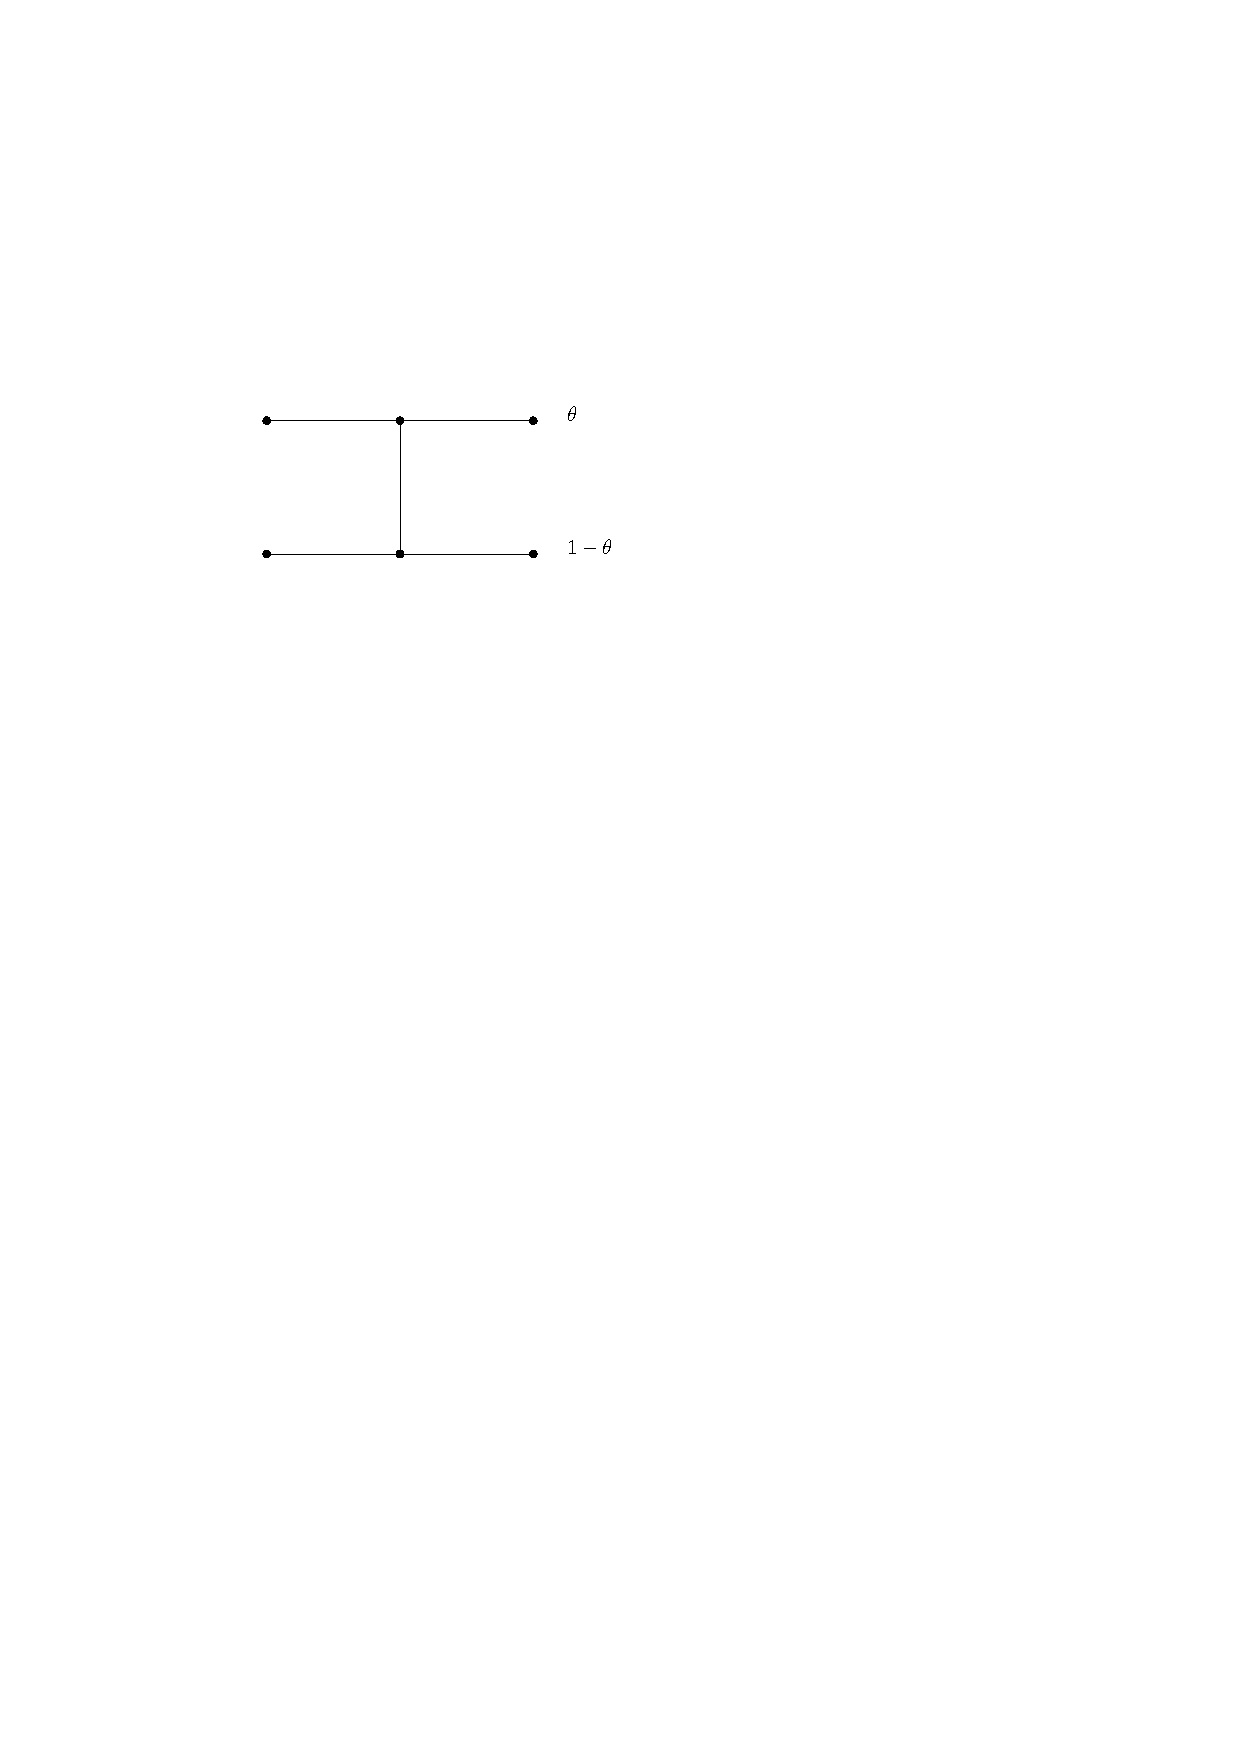
\includegraphics[width=0.5\linewidth]{pic1}
  \caption{Расположение узлов разностной схемы}\label{ris:1}
\end{figure}

Разностная схема для задачи  \eqref{eq:5}-\eqref{eq:8}:
\begin{align}
        &-\Ap{A}{i} \Ap{u}{i-1} + \Ap{C}{i} \Ap{u}{i} - \Ap{B}{i} \Ap{u}{i+1} = \Ap{F}{i}, \;\; i = \overline{1,N_{x}-1}, \label{eq:9.0}\\
        &u^0_i = u_{0i}, \label{eq:9.1}\\
        &\Ap{u}{0} = \Ap{\varkappa}{1} \Ap{u}{1} + \Ap{\nu}{1},\;\; \Ap{u}{N_{x}} = \Ap{\varkappa}{2} \Ap{u}{N_{x} -1} + \Ap{\nu}{2}, \label{eq:9.2}
\end{align}
\begin{align}
        &\Ap{A}{i} = \theta \Ap{\alpha}{i - \frac{1}{2}}, \label{eq:10.1}\\
        &\Ap{C}{i} = 1 + \theta \left(\Ap{\alpha}{i + \frac{1}{2}} + \Ap{\alpha}{i - \frac{1}{2}}\right), \label{eq:10.2}\\
        &\Ap{B}{i} = \theta \Ap{\alpha}{i + \frac{1}{2}}, \label{eq:10.3}\\
        &\Ap{F}{i} = (1 - \theta) \Apr{\alpha}{i - \frac{1}{2}} \Apr{u}{i-1} + \SR{1 - (1 - \theta) \left(\Apr{\alpha}{i + \frac{1}{2}} + \Apr{\alpha}{i - \frac{1}{2}}\right)} \Apr{u}{i} + (1 - \theta) \Apr{\alpha}{i + \frac{1}{2}} \Apr{u}{i+1} + \tau f_{i}^{j}, \label{eq:10.4}\\
        &\Ap{\varkappa}{1} = 0, \;\; \Ap{\varkappa}{2} = 1, \;\; \Ap{\nu}{1} = \Ap{\nu}{2} = 0, \label{eq:10.5}
\end{align}
где $\displaystyle \alpha(x) = \frac{\tau}{h^2} D(x)$.

Для решения трёхточечных разностных уравнений вида \eqref{eq:9.0} с краевыми условиями \eqref{eq:9.2} применяется метод прогонки.

Формулы прямой прогонки:
\begin{align}
        &\Ap{\xi}{i+1} = \frac{\Ap{B}{i}}{\Ap{C}{i} - \Ap{A}{i} \Ap{\xi}{i}},\;\; \Ap{\xi}{1} = \Ap{\varkappa}{1},\;\; i = \overline{1,N_{x} - 1}, \label{eq:11}\\
        &\Ap{\eta}{i+1} = \frac{\Ap{A}{i} \Ap{\eta}{i} + \Ap{F}{i}}{\Ap{C}{i} - \Ap{\xi}{i} \Ap{A}{i}}, \;\; \Ap{\eta}{1} = \Ap{\nu}{1},\;\; i = \overline{1,N_{x} - 1}. \label{eq:12}
\end{align}

Формулы обратной прогонки:
\begin{align}
        &\Ap{u}{N_x} = \frac{\Ap{\nu}{2} + \Ap{\varkappa}{2} \Ap{\eta}{N_{x}}}{1 - \Ap{\varkappa}{2} \Ap{\xi}{N_{x}}}, \label{eq:16}\\
        &\Ap{u}{i} = \Ap{\xi}{i+1} \Ap{u}{i+1} + \Ap{\eta}{i+1}, \;\; i = \overline{N_{x}-1, 0}. \label{eq:17}
\end{align}

\newpage
\section{Постановка задачи}
Найти функцию $u(x,t)$, являющуюся решением уравнения
\begin{equation}\label{eq:18}
  \PartDif{u}{t} = a^2 \PartDiff{u}{x} + \cos(x), ~~ a=0.3,
\end{equation}
в области $\{0\;<\;x\;<\;l=2\pi,~0\;<\;t\;<T=2\}$ с начальными и граничными условиями
\begin{align}
        &u(x,0) = \sin\left(\frac{x}{2}\right) + \frac{x}{2}, \label{eq:19}\\
        &u(0,t) = 0, ~~ \PartDif{u}{x}(l,t) = 0. \label{eq:20}
\end{align}

Решить краевую задачу явным и неявным методом. При решении задач с использованием явной схемы получить решение, соблюдая условие устойчивости и нарушив его. Построить трёхмерные графики распределения температур.

\section{Результаты}
\begin{figure}[htbp]
  \centering
  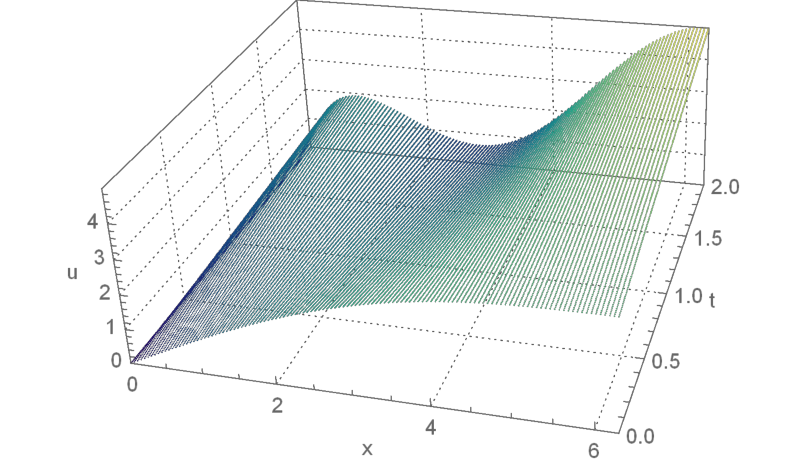
\includegraphics[width=1\linewidth]{vis_imp}
  \caption{Численное решение при использовании неявной схемы}\label{}
\end{figure}

Условие устойчивости явной схемы ($\theta = 0$):
$$K = \frac{a^2 \tau}{h^2} \leq \frac{1}{2}$$

\begin{figure}[htbp]
  \centering
  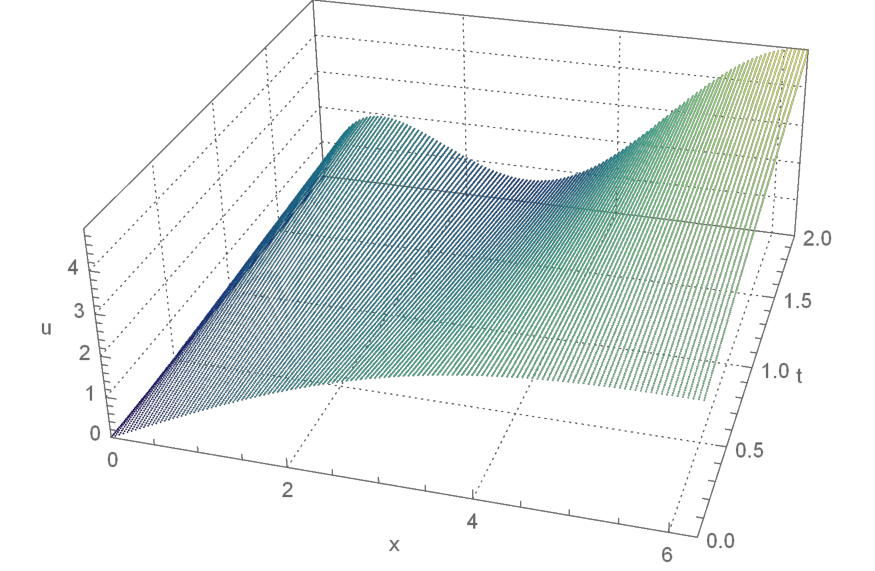
\includegraphics[width=1\linewidth]{vis_exp_1}
  \caption{Численное решение при использовании явной схемы с выполненным условием устойчивости $K = 0.36$}\label{}
\end{figure}

\begin{figure}[htbp]
  \centering
  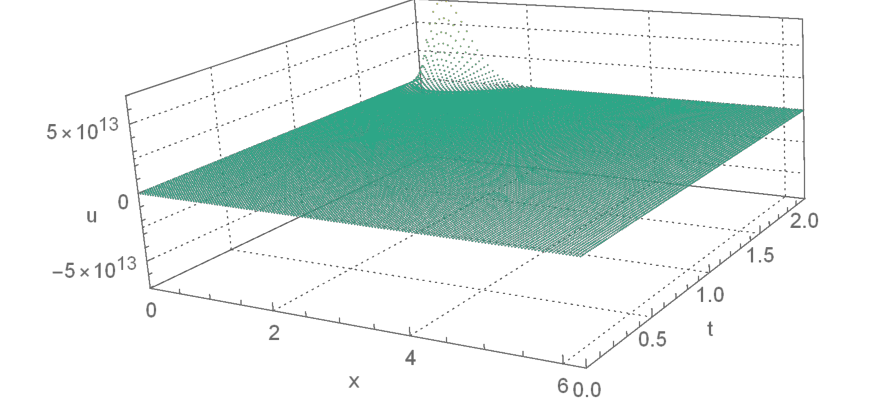
\includegraphics[width=1\linewidth]{vis_exp_2}
  \caption{Численное решение при использовании явной схемы с невыполненным условием устойчивости $K = 0.57$}\label{}
\end{figure}

\section{Вывод}
Решена краевая задача явным и неявным методами. При решении задач с использованием явной схемы получены решения, соблюдая условие устойчивости и нарушив его. Построены трёхмерные графики распределения температур.

При нарушении условия устойчивости явной схема решение, полученное при ее применении <<разваливается>>.
\end{document} 